

\section{Experiments}

In this section, we evaluate the effect of reducing parameter variance on generalization behavior. Lemma \ref{lem: factorising_interpetation} bounds $w(\omega)$ by upper- and lower bounding the weight of the combinations of variables across the domains $[n]$ and $[\bar{n}]$ with $M_{max}$ and $M_{min}$. In practice, for almost all worlds, this bound is loose. This is because not all $k$-tuples chosen from across the domains will have the extreme weights. Therefore, it is more effective to reduce the spread between all the weights, rather than merely scaling the upper and the lower bound. Also note that for most MLNs, for some $\omega \in \Omega^{k}$, we will have that $w_{k}(\omega)=1$, i.e., none of the formulas in the MLN will be realized on $\omega$. Thus, in most practical cases,  to reduce the spread of the weights $a_i$, one should reduce their spread around $0$.

Multiple approaches discussed in the literature, directly or indirectly, minimize the parameter variance  \cite{huynh2008discriminative,DA_MLN}. We empirically evaluated the effects of three such approaches: L1 regularization, L2 regularization, and Domain-Size Aware Markov Logic Networks (DA-MLNs) \cite{DA_MLN}. 
Both L1 and L2 regularization directly work to reduce the spread of the parameters: L1 regularization penalizes the sum of the absolute weight values and L2 regularization penalizes the sum of squared weights. A DA-MLN is an adaptation of a regular MLN that achieves the same effect by down-scaling formula weights depending on the test set domain size:

\begin{equation}
\label{eq: MLN}
    P^{(n)}_{\Phi}(\omega) = \frac{1}{Z(n)}\exp\Bigl(\sum_{(\phi_i,a_i)\in \Phi}\frac{a_i}{s_i} N(\phi_i,\omega)\Bigr)
\end{equation}
The scale-down factor $s_i$ is defined as follows:
\begin{align}
   s_i =  \underset{P \in \phi_i}{\max}\Bigl( \max\bigl(1,\underset{x \in Vars_{\phi_i}(P)^-}{\prod} \lvert\Delta_x\rvert\bigr)\Bigr)
\end{align}
where $\lvert \Delta_x \rvert$ is the test set domain size of $x$ and $Vars_{\phi_i}(P)^-$ is the set of logical variables appearing in $\phi_i$ but not in $P$.

To precisely verify our theoretical results, we employed Lifted Inference \cite{kersting2012lifted,First_Order_Prob_Inf} and Lifted Generative Learning \cite{vanHaaren2016} methods, which calculate the exact dataset likelihood. 

%In contrast, alternative methods optimize approximate objectives, such as pseudo-likelihood \cite{besag1975statistical}, which may interfere with the verification of the theoretical results. 

%All our experiments were run on an Intel Core i9-11900KF with 8 cores and 64gb of RAM.

\subsection{Datasets}

To provide a thorough analysis of the effects of different methods for generalizing across different domain sizes we used four datasets commonly used in related literature: Friends \& Smokers (FS) \cite{singla2008}, IMDB\footnote{\label{note2}Dataset available on the Alchemy website: \href{https://alchemy.cs.washington.edu/data/}{https://alchemy.cs.washington.edu/data/}} \cite{mihalkova2007}, WebKB\footnoteref{note2} \cite{mihalkova2007} and Nations\footnoteref{note2} \cite{rummel1992}.\\
%\footnote{\label{note1}Dataset available on the Forclift repository: \href{https://github.com/UCLA-StarAI/Forclift}{https://github.com/UCLA-StarAI/Forclift}}
\\
\noindent \textbf{Friends \& Smokers (FS).} This synthetic dataset captures information about smoking habits, friendships, and cancer diagnoses of a set of people. The data was created in a way to model real-life communities \cite{DA_MLN}: First, a population was split into groups and each group was with probability $0.3$ labeled to be a "Smoking"-group, or labeled a "Non-Smoking"-group otherwise. Based on their group membership, individuals were then with a certain probability assigned to be smokers: $0.7$ for "Smoking"-groups, $0.1$ for "Non-Smoking"-groups. Next, some individuals were chosen to suffer from cancer. For smokers, the probability of being chosen was set to $0.5$, for non-smokers it was set to $0.1$. Lastly, friendships were assigned based on the group partitioning, with a $0.8$ probability for intra-group friendships, and a $0.1$ probability for inter-group friendships. For our experiments, we generated a test dataset of size 500.\\
%We generated test datasets of sizes varying from 100 to 500.\\
\\
\noindent \textbf{IMDB.} Taken from the International Movie Database this dataset contains information about movies and their actors and directors. Also included are certain attributes like gender and work relations of actors and directors. The dataset has a total of 297 constants, of which 268 are of type person, and 6 predicates.\\
\\
\noindent \textbf{WebKB.} This dataset captures information about web pages from four US universities. For each web page, the original dataset \cite{craven2001} includes a label (e.g. Course, Faculty) as well as textual information about the page contents. Similar to Mihalkova et al. \cite{mihalkova2007}, the version we use disregards the textual information and focuses on page classes and relations, for example between courses and teaching assistants. This version of the dataset comprises a total of 989 constants, of which 746 are of type person, and 5 predicates.\\
\\
%\subsubsection{UW-CSE.} Comprising of information about the University of Washington CSE Department this dataset contains information modeling relations between students, professors, classes, and publications. Such relations include \texttt{AdvisedBy} and \texttt{Ta}. The dataset includes a total of 770 constants and 9 predicates.
\noindent \textbf{Nations.} This dataset contains a set of features of nations and relations between them. Relations include treaties and (economic-)aid, features include governance types and technological advancements. In total, there are 14 nations, 111 features, and 56 relations.

\subsection{Methodology}

The structures of the MLNs we used were adopted from Van Haaren et al. \cite{vanHaaren2016}, who introduced a Lifted Structure Learning (LSL) approach. LSL ensures that the learned structures are liftable and learnable in practice. For the Nations dataset, which, with over 160 predicates, characterizes an infeasibly large search space of possible clauses for LSL, we used a hand-crafted MLN of 50 formulas with intuitive meaning. For weight learning, we employed Lifted Generative Learning \cite{vanHaaren2016}. This allows us to compare the exact test-dataset likelihoods, which is the natural evaluation measure for generative learning \cite{darwiche2009modeling,koller2009probabilistic,murphy2012machine,vanHaaren2016} and is also best suited for validating our theoretical results.

To evaluate generalization across varying domain sizes we generated 20 training samples for weight learning and 5 test samples for each of the tested sizes. For generating the training samples, we uniformly sampled subsets from a specific type of constant: person for FS, IMDB, and WebKB, and nation for the corresponding Nations dataset. We then constructed the subgraph induced by these subsets by adding all ground atoms where the contained domain constants of the sampled domain type are a subset of the sampled constants. The process for generating test samples followed a similar approach.

%, with the exception of the FS dataset, where we were able to generate them directly.

\textcolor{red}{How do we do training?}
\textcolor{red}{Compare Regularization with No Regularization}
\textcolor{red}{Measures we calculate: For each training sample train MLN run inference for each test sample take delta to no reg}

\subsection{Results}

\begin{figure}
     \centering
     \begin{subfigure}[b]{0.49\textwidth}
         \centering
         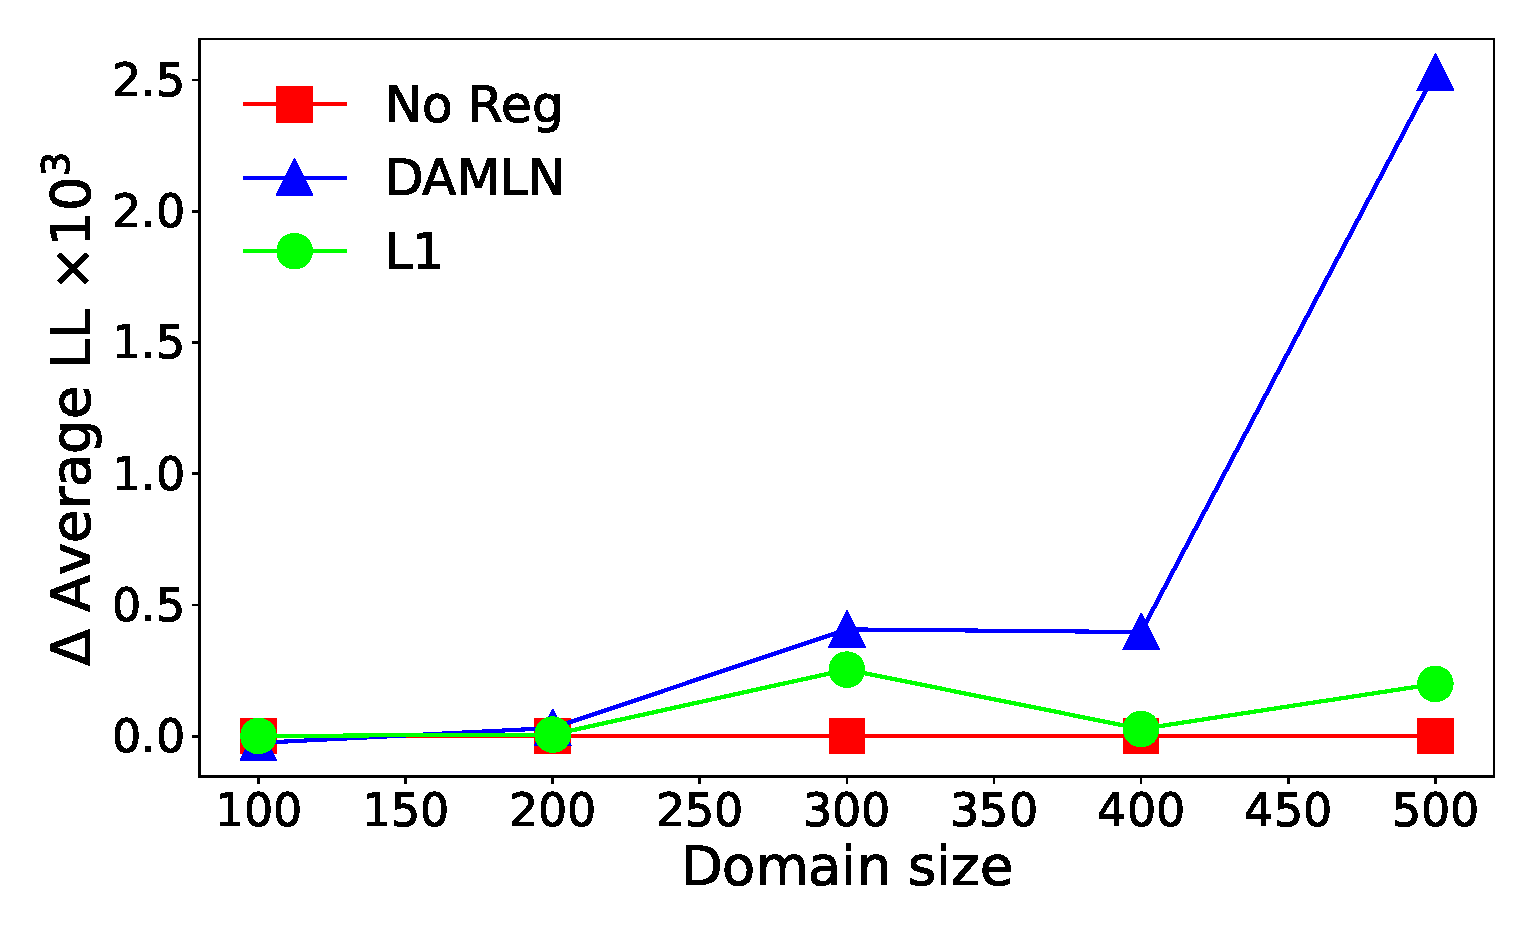
\includegraphics[width=\textwidth]{smoking_likelihoods_mean.eps}
         \caption{$\Delta$-Likelihoods (FS)}
         \label{Likelihoods (FS)}
     \end{subfigure}
     \hfill
     \begin{subfigure}[b]{0.49\textwidth}
         \centering
         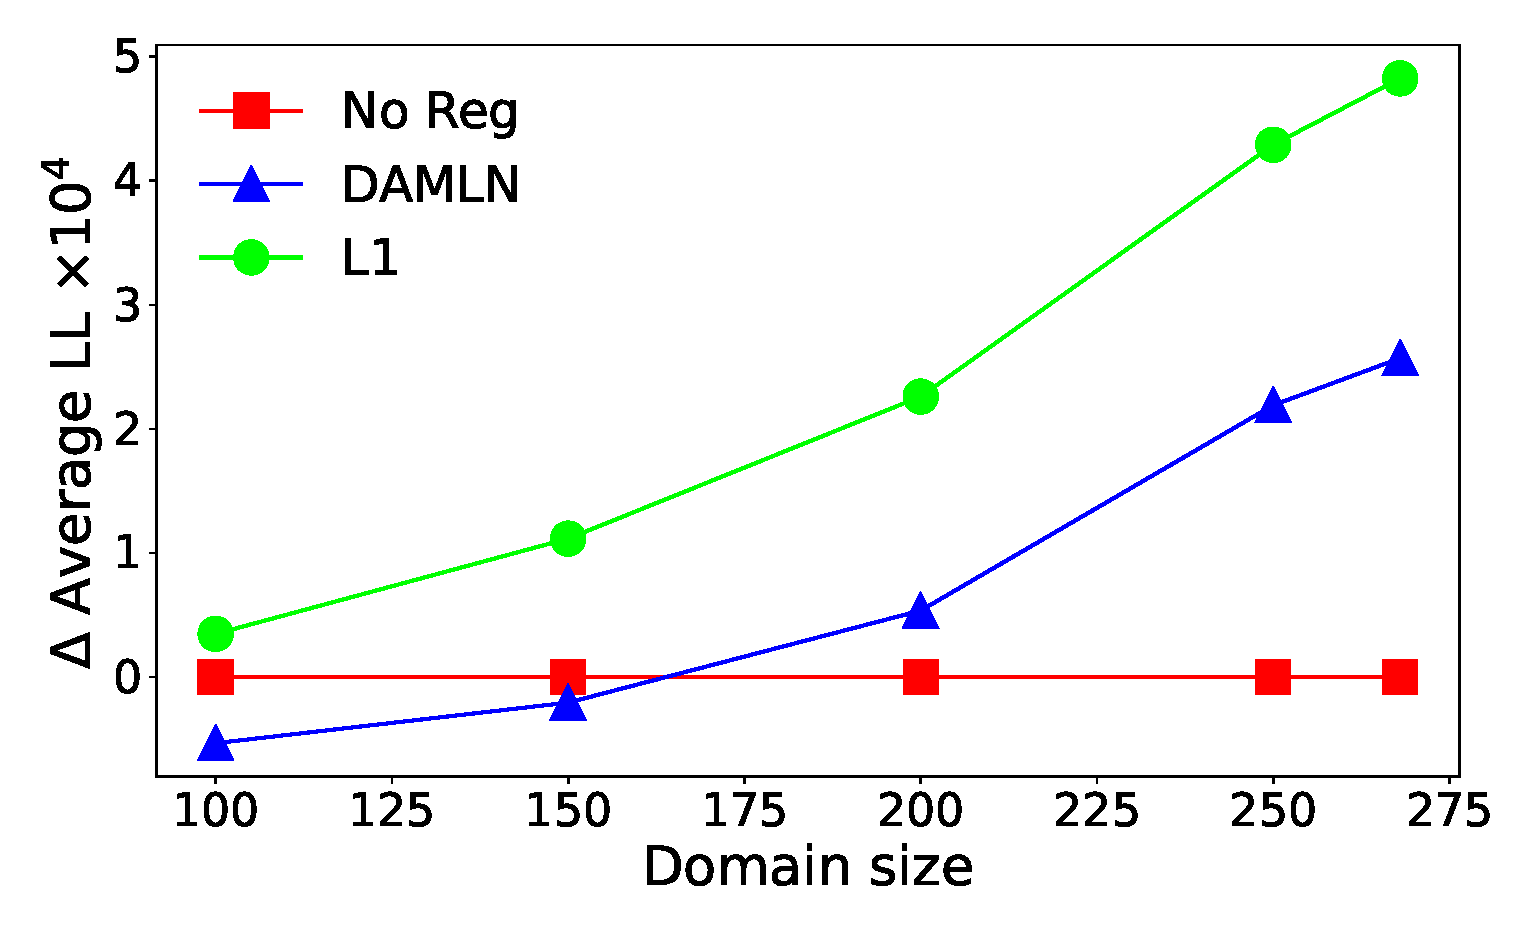
\includegraphics[width=\textwidth]{imdb_likelihoods_mean.eps}
         \caption{$\Delta$-Likelihoods (IMDB)}
         \label{Likelihoods (IMDB)}
     \end{subfigure}
     \hfill
     \begin{subfigure}[b]{0.49\textwidth}
         \centering
         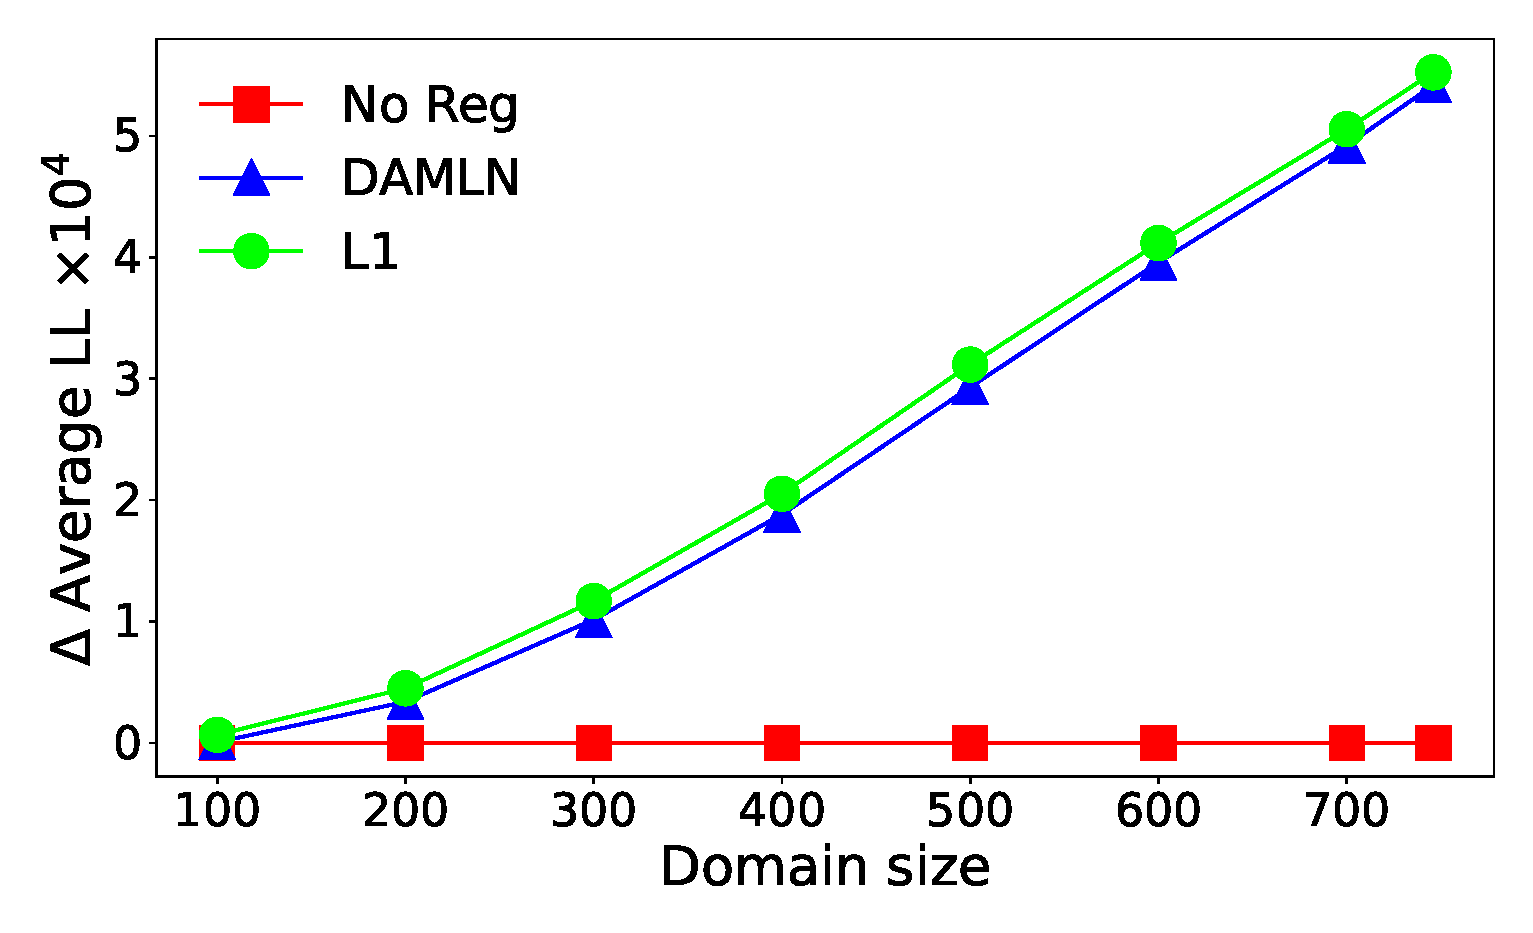
\includegraphics[width=\textwidth]{webkb_likelihoods_mean.eps}
         \caption{$\Delta$-Likelihoods (WebKB)}
         \label{Likelihoods (WebKB)}
     \end{subfigure}
     \begin{subfigure}[b]{0.49\textwidth}
         \centering
         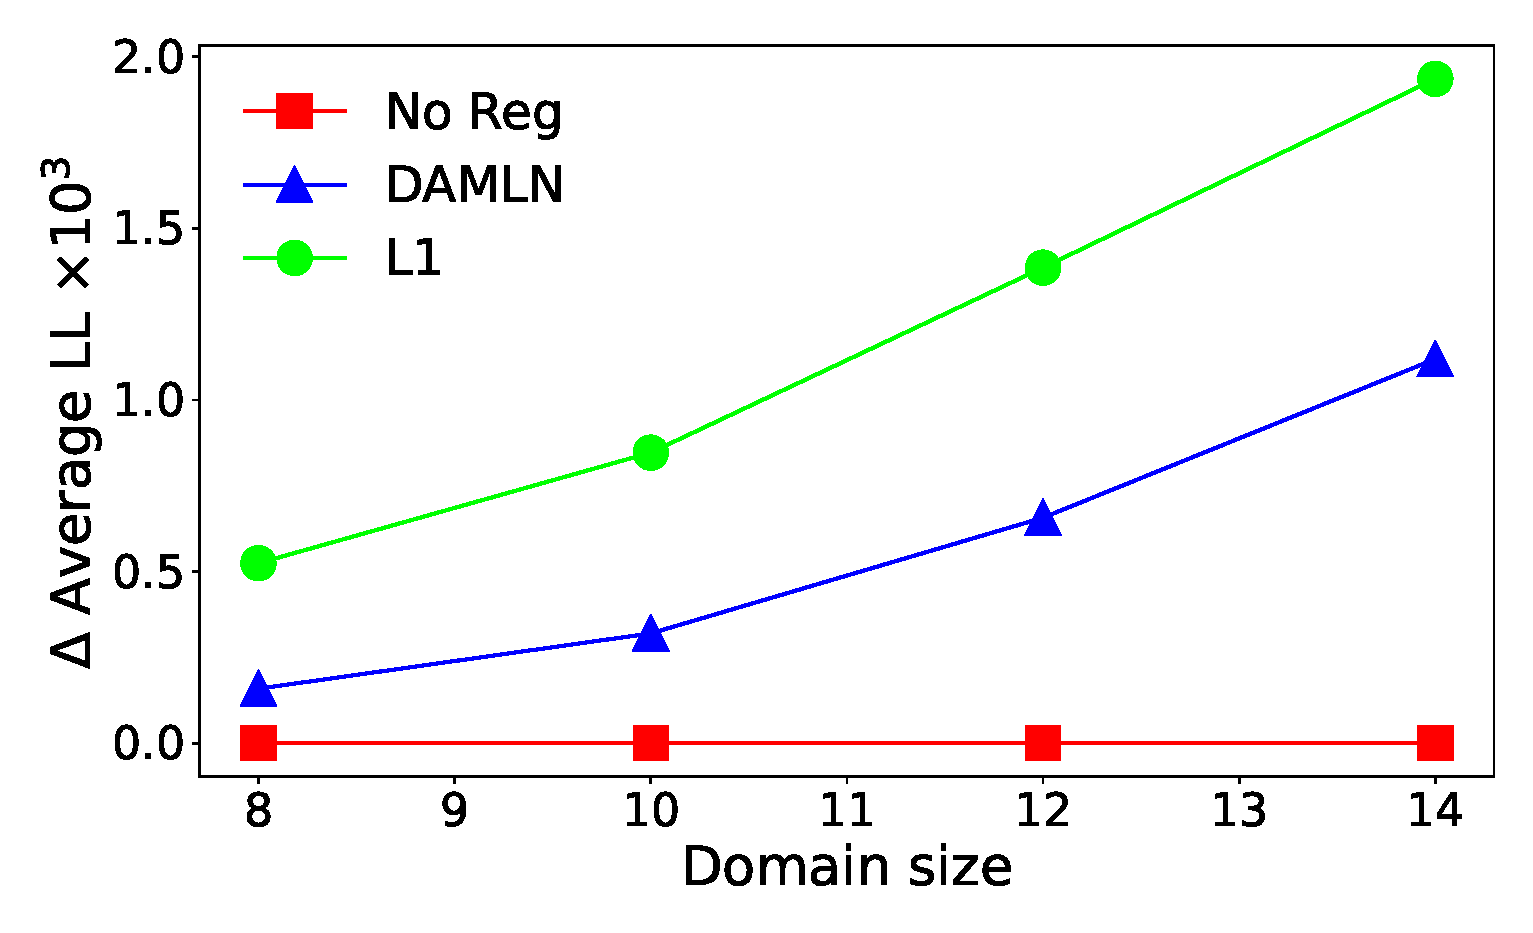
\includegraphics[width=\textwidth]{nations_likelihoods_mean.eps}
         \caption{$\Delta$-Likelihoods (Nations)}
         \label{Likelihoods (Nations)}
     \end{subfigure}
        \caption{Results for the Friends \& Smokers, IMDB, WebKB, and Nations datasets}
        \label{fig:three graphs}
\end{figure}

Discuss the phenomenon with all negative groundings which helps performance of regularization

